\chapter{Introduction}
\section{Problem Description}
In this project, we are expected to create a RISC-V pipelined datapath simulator on a high level programming language. Simulation is expected to implement hazard control and forwarding units as discussed throughout the lectures and in the course textbook. Simulation is also expected to keep data on CPI, total clock cycles, total number of stalls, stalls caused by instructions and prepare an output report on the execution using that data. Figure \ref{fig:datapath} is the diagram for the pipelined datapath structure taken from the course textbook. The simulator is also expected to simulate the instructions and, or, sub, add, beq, sd and ld. \\

\href{https://drive.google.com/drive/folders/104gLuhNgoEN1hMbGKwAH2UXVvRCwPsN0}{\color{blue}{GOOGLE DRIVE LINK FOR THE CODE}}
\begin{figure}
    \centering
    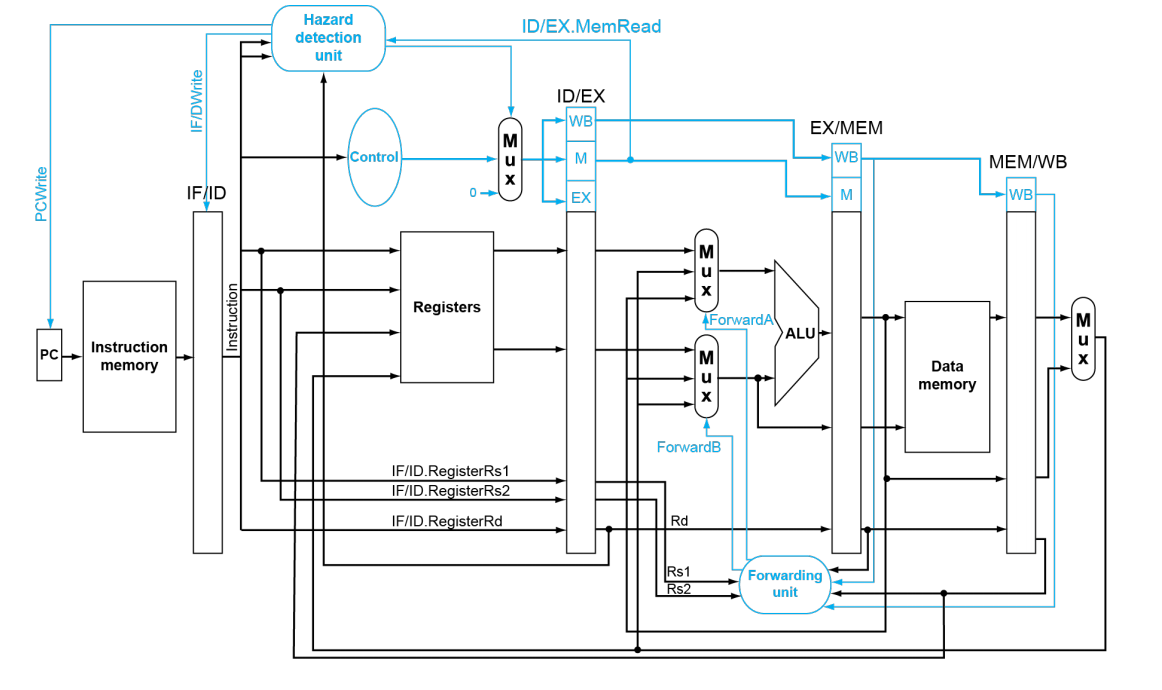
\includegraphics[scale=0.5]{1.png}
    \caption{Pipelined datapath diagram taken from course textbook}
    \label{fig:datapath}
\end{figure}

\section{Our Approach}
We have decided to write this simulator in the programming language Python. We aimed create a simulator structure that is strongly correlated with both the data and logical structure of the datapath. Simulator program, via a console argument, takes a plain text file that contains assembly code and some data initialization and fill the code in its virtual memory. Our simulator can run add. sub, and, or, beq, ld and sd instructions. Our simulator has variables for all the registers of RISC-V ISA and also for registers like ID/EX etc. We used the standard data structures of Python such as dictionaries and lists to simulate registers and memory. And to simulate the execution, we have defined methods for each phase of the datapath that are continuously executed one by one until the program counter reaches the end of the code. Those methods(for example a method for simulating the ID phase), during their execution, update the related registers according to their function. During the execution, simulator keeps all the related statistics to create a final report.


